\documentclass[a4paper,12pt]{article} 

%%% Работа с русским языком
\usepackage{cmap}					% поиск в PDF
\usepackage{mathtext} 				% русские буквы в фомулах
\usepackage[T2A]{fontenc}			% кодировка
\usepackage[utf8]{inputenc}			% кодировка исходного текста
\usepackage[english,russian]{babel}	% локализация и переносы

%%% Дополнительная работа с математикой
\usepackage{amsmath,amsfonts,amssymb,amsthm,mathtools, gensymb} % AMS
\usepackage{icomma} % "Умная" запятая: $0,2$ --- число, $0, 2$ --- перечисление

%%Таблица
\usepackage[table,xcdraw]{xcolor}
\usepackage{caption}
\usepackage{subcaption}
\usepackage{floatrow}
\floatsetup[table]{capposition=top}
\floatsetup[wrapfigure]{capposition=bottom}
%multi-column
%\usepackage{multi-column}
%multi-row
\usepackage{multirow}


%% Номера формул
\mathtoolsset{showonlyrefs=true} % Показывать номера только у тех формул, на которые есть \eqref{} в тексте.

%% Шрифты
\usepackage{euscript}	 % Шрифт Евклид
\usepackage{mathrsfs} % Красивый матшрифт

%% Свои команды
\DeclareMathOperator{\sgn}{\mathop{sgn}}

%% Перенос знаков в формулах (по Львовскому)
\newcommand*{\hm}[1]{#1\nobreak\discretionary{}
{\hbox{$\mathsurround=0pt #1$}}{}}

%% Стиль страницы
\usepackage{fancyhdr}

%% Для рисунков
\usepackage{graphicx}
\usepackage[export]{adjustbox}
\usepackage{float}
\usepackage{ragged2e}
\usepackage{wrapfig}

%Отступы и поля 
\textwidth=20cm
\oddsidemargin=-2cm
\topmargin=-2cm
\textheight=25cm

\pagestyle{fancy}
\begin{document}
\begin{titlepage}
\begin{center}
%\vspace*{1cm}
\large{\small ФЕДЕРАЛЬНОЕ ГОСУДАРСТВЕННОЕ АВТОНОМНОЕ ОБРАЗОВАТЕЛЬНОЕ\\ УЧРЕЖДЕНИЕ ВЫСШЕГО ОБРАЗОВАНИЯ \\ МОСКОВСКИЙ ФИЗИКО-ТЕХНИЧЕСКИЙ ИНСТИТУТ\\ (НАЦИОНАЛЬНЫЙ ИССЛЕДОВАТЕЛЬСКИЙ УНИВЕРСИТЕТ)\\ ФАКУЛЬТЕТ АЭРОКОСМИЧЕСКИХ ТЕХНОЛОГИЙ}
\vfill
\line(1,0){430}\\[1mm]
%\huge{Лабораторная 2}\\
\huge\textbf{Ползучесть материалов}\\
\line(1,0){430}\\[1mm]
\vfill
\begin{flushright}
\normalsize{Рогозин Владимир}\\
\normalsize{\textbf{Группа Б03-106}}\\
\end{flushright}
\end{center}
\end{titlepage}
\fancyhead[c] {Ползучесть материалов}

\textbf{Цель работы:} 

1) Проверить линейность ползучести материала. 

2) Проверить принцип суперпозиции Больцмана для линейно ползучих материалов.

\textbf{Теоретические сведения:} 

Способность материала деформироваться под действием постоянных напряжений называется \textit{ползучестью}. 

Результаты испытаний при одноосном растяжении представляются в виде \textit{кривых ползучести} -- кривых зависимости деформации от времени. 

С увеличением времени наблюдается возрастание деформации при постоянном уровне напряжений. Полная деформация образца в момент времени $t'$ определяется суммой упругой деформации $\varepsilon^у (t_0)$ и \textit{деформацией ползучести} $\varepsilon^п (t')$:
\[\varepsilon (t') = \varepsilon^у (t_0) + \varepsilon^п (t') = \frac{\sigma}{E} + \Pi (\sigma, t_0, t'),\]
где $\Pi$ -- \textit{функция ползучести}, $E$ -- модуль Юнга.

Если увеличение деформаций ползучести пропорционально увеличению напряжений, то говорят о \textit{линейной ползучести}, в противном случае -- о \textit{нелинейной ползучести}.

При линейной ползучести кривые, полученные при разных уровнях напряжений, оказываются подобными. Это означает, что деформация ползучести может быть найдена как произведение двух функций: одна из которых зависит только от напряжения, вторая -- только от времени.
\[\varepsilon (t) = \frac{\sigma}{E} + \Pi (t, t_0) \sigma.\]

В некоторых материалах наблюдаются изменения механических свойств во времени при неизменных условиях. Это явление получило условное название \textit{<<старение>>}. Деформация ползучести при <<старении>> зависит не только от уровня и продолжительности действия нагрузки, но и от момента её приложения (возраста материала).

Ползучесть нестареющих материалов зависит только от уровня напряжения и продолжительности его действия, и не зависит от момента приложения нагрузки. 

У нестареющих материалов функция ползучести $\Pi$ будет разностного типа:
\[\varepsilon (t) = \frac{\sigma}{E} + \Pi (t - t_0) \sigma.\]

В силу линейности задачи (если рассматривать только линейную ползучесть) для получения зависимости между переменными напряжениями и и деформациями важное значение имеет \textit{принцип суперпозиции Больцмана.} Согласно ему суммарная деформация ползучести при переменном напряжении может быть найдена как сумма деформаций ползучести, вызванных соответствующими приращениями напряжений. Величина деформации ползучести $\Delta \varepsilon^n$ зависит от величины приращения напряжений $\Delta \sigma$ и продолжительности его действия, но не зависит то величины и длительности действия других приращений.
\[\varepsilon (t_4) = \frac{\sigma (t_4)}{E} + \Pi (t_4 - t_0) \Delta \sigma_1 + \Pi (t_4 - t_1) \Delta \sigma_2 + \Pi (t_4 - t_2) \Delta \sigma_3 + \Pi (t_4 - t_3) \Delta \sigma_4.\]
Если изменение напряжения протекает по непрерывной кривой, то суммирование заменяется интегрированием
\[\varepsilon (t) = \frac{\sigma (t)}{E} + \int\limits_0^t \Pi (t - \tau) d\sigma (\tau),\]
где $t$ -- момент наблюдения, $\tau$ -- текущее время.
\begin{figure}[H]\label{fig: Linear Polz}
    \centering
    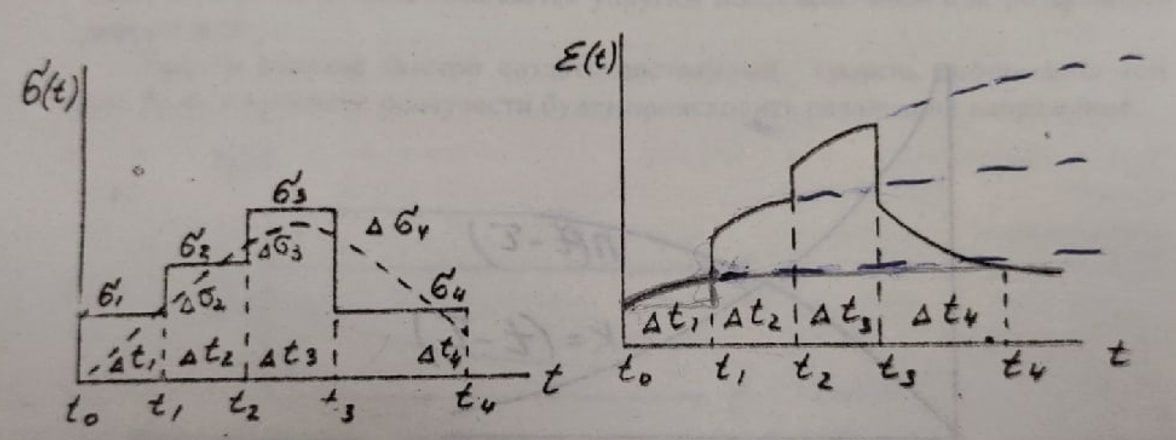
\includegraphics[width = \textwidth]{Линейность ползучести.png}
    \caption{Пример ступенчатого и непрерывного нагружения}
\end{figure}

Преобразуем подынтегральное выражение, для этого вычислим интеграл по частям:
\[\varepsilon (t) = \frac{\sigma (t)}{E} + \Pi (t - \tau) \sigma (\tau)\bigg|_0^t - \int\limits_0^t \frac{\partial}{\partial t} \Pi (t - \tau) \sigma (\tau) d\tau,\]
при $\tau = 0$, $\sigma (0) = 0$; при $\tau = t$, $\Pi (t - \tau) = 0$, отсюда получаем
\[\varepsilon (t) = \frac{\sigma (t)}{E} + \int\limits_0^t k(t - \tau) \sigma (\tau) d\tau,\]
где $k(t - \tau) = - \partial \Pi (t - \tau) / \partial t$ -- \textit{ядро ползучести} или \textit{функция влияния}.

В простейшем случае, функцию ползучести можно представить выражением 
\[\Pi (t - \tau) = A - A \exp\{-\alpha (t - \tau)\}.\]

В данной работе будем использовать немного другое выражение для функции ползучести, а именно
\[\Pi (t - \tau) = A - B \exp\{-\alpha (t - \tau) - C \exp\{-\beta (t - \tau)\},\]
причём стоит заметить, что $A = B + C$, так как $\Pi (0) = 0$.

\textbf{Обработка данных:} Параметры установки: $b = 19,6$ мм, $d = 5,6$ мм, $S = b \cdot d$; $l_0 = 50$ мм. Будем снимать зависимость удлинениния от времени в течение 20-ти минут. После первых 10-ти минут увеличим силу примерно в два раза. Результаты измерений представлены в таблице ниже. По данным из таблицы построим графики зависимости деформации и напряжения от времени.

\begin{table}[H]\label{tab: data eps(t)}
    \centering
    \begin{tabular}{|
        >{\columncolor[HTML]{FFFFFF}}c 
        >{\columncolor[HTML]{FFFFFF}}c 
        >{\columncolor[HTML]{FFFFFF}}c |
        >{\columncolor[HTML]{FFFFFF}}c 
        >{\columncolor[HTML]{FFFFFF}}c 
        >{\columncolor[HTML]{FFFFFF}}c |}
        \hline
        \multicolumn{3}{|c|}{\cellcolor[HTML]{FFFFFF}{\color[HTML]{000000} $F_1 = 30,5$ Н}} &
          \multicolumn{3}{c|}{\cellcolor[HTML]{FFFFFF}{\color[HTML]{000000} $F_2 = 60,8$}} \\ \hline
        \multicolumn{1}{|c|}{\cellcolor[HTML]{FFFFFF}{\color[HTML]{000000} $t$, мин}} &
          \multicolumn{1}{c|}{\cellcolor[HTML]{FFFFFF}{\color[HTML]{000000} $\Delta l$, мм}} &
          {\color[HTML]{000000} $\varepsilon^п$} &
          \multicolumn{1}{c|}{\cellcolor[HTML]{FFFFFF}{\color[HTML]{000000} $t$, мин}} &
          \multicolumn{1}{c|}{\cellcolor[HTML]{FFFFFF}{\color[HTML]{000000} $\Delta l$, мм}} &
          {\color[HTML]{000000} $\varepsilon^п$} \\ \hline
        \multicolumn{1}{|c|}{\cellcolor[HTML]{FFFFFF}{\color[HTML]{000000} 0}} &
          \multicolumn{1}{c|}{\cellcolor[HTML]{FFFFFF}{\color[HTML]{000000} 0.2615}} &
          {\color[HTML]{000000} 0} &
          \multicolumn{1}{c|}{\cellcolor[HTML]{FFFFFF}{\color[HTML]{000000} 10}} &
          \multicolumn{1}{c|}{\cellcolor[HTML]{FFFFFF}{\color[HTML]{000000} 0,7280}} &
          {\color[HTML]{000000} 0,004136} \\ \hline
        \multicolumn{1}{|c|}{\cellcolor[HTML]{FFFFFF}{\color[HTML]{000000} 0,5}} &
          \multicolumn{1}{c|}{\cellcolor[HTML]{FFFFFF}{\color[HTML]{000000} 0,2845}} &
          {\color[HTML]{000000} 0,00046} &
          \multicolumn{1}{c|}{\cellcolor[HTML]{FFFFFF}{\color[HTML]{000000} 11}} &
          \multicolumn{1}{c|}{\cellcolor[HTML]{FFFFFF}{\color[HTML]{000000} 0,8231}} &
          {\color[HTML]{000000} 0,006038} \\ \hline
        \multicolumn{1}{|c|}{\cellcolor[HTML]{FFFFFF}{\color[HTML]{000000} 1}} &
          \multicolumn{1}{c|}{\cellcolor[HTML]{FFFFFF}{\color[HTML]{000000} 0,2938}} &
          {\color[HTML]{000000} 0,000646} &
          \multicolumn{1}{c|}{\cellcolor[HTML]{FFFFFF}{\color[HTML]{000000} 12}} &
          \multicolumn{1}{c|}{\cellcolor[HTML]{FFFFFF}{\color[HTML]{000000} 0,8714}} &
          {\color[HTML]{000000} 0,007004} \\ \hline
        \multicolumn{1}{|c|}{\cellcolor[HTML]{FFFFFF}{\color[HTML]{000000} 2}} &
          \multicolumn{1}{c|}{\cellcolor[HTML]{FFFFFF}{\color[HTML]{000000} 0,3031}} &
          {\color[HTML]{000000} 0,000832} &
          \multicolumn{1}{c|}{\cellcolor[HTML]{FFFFFF}{\color[HTML]{000000} 13}} &
          \multicolumn{1}{c|}{\cellcolor[HTML]{FFFFFF}{\color[HTML]{000000} 0,9029}} &
          {\color[HTML]{000000} 0,007634} \\ \hline
        \multicolumn{1}{|c|}{\cellcolor[HTML]{FFFFFF}{\color[HTML]{000000} 3}} &
          \multicolumn{1}{c|}{\cellcolor[HTML]{FFFFFF}{\color[HTML]{000000} 0,3123}} &
          {\color[HTML]{000000} 0,001016} &
          \multicolumn{1}{c|}{\cellcolor[HTML]{FFFFFF}{\color[HTML]{000000} 14}} &
          \multicolumn{1}{c|}{\cellcolor[HTML]{FFFFFF}{\color[HTML]{000000} 0,9278}} &
          {\color[HTML]{000000} 0,008132} \\ \hline
        \multicolumn{1}{|c|}{\cellcolor[HTML]{FFFFFF}{\color[HTML]{000000} 5}} &
          \multicolumn{1}{c|}{\cellcolor[HTML]{FFFFFF}{\color[HTML]{000000} 0,3214}} &
          {\color[HTML]{000000} 0,001198} &
          \multicolumn{1}{c|}{\cellcolor[HTML]{FFFFFF}{\color[HTML]{000000} 15}} &
          \multicolumn{1}{c|}{\cellcolor[HTML]{FFFFFF}{\color[HTML]{000000} 0,9465}} &
          {\color[HTML]{000000} 0,008506} \\ \hline
        \multicolumn{1}{|c|}{\cellcolor[HTML]{FFFFFF}{\color[HTML]{000000} 9}} &
          \multicolumn{1}{c|}{\cellcolor[HTML]{FFFFFF}{\color[HTML]{000000} 0,3336}} &
          {\color[HTML]{000000} 0,001442} &
          \multicolumn{1}{c|}{\cellcolor[HTML]{FFFFFF}{\color[HTML]{000000} 19}} &
          \multicolumn{1}{c|}{\cellcolor[HTML]{FFFFFF}{\color[HTML]{000000} 1,0080}} &
          {\color[HTML]{000000} 0,009736} \\ \hline
        \multicolumn{1}{|c|}{\cellcolor[HTML]{FFFFFF}{\color[HTML]{000000} 10}} &
          \multicolumn{1}{c|}{\cellcolor[HTML]{FFFFFF}{\color[HTML]{000000} 0,3367}} &
          {\color[HTML]{000000} 0,001504} &
          \multicolumn{1}{c|}{\cellcolor[HTML]{FFFFFF}{\color[HTML]{000000} 20}} &
          \multicolumn{1}{c|}{\cellcolor[HTML]{FFFFFF}{\color[HTML]{000000} 1,0142}} &
          {\color[HTML]{000000} 0,009860} \\ \hline
    \end{tabular}
    \caption{Данные измерений удлинения от времени}
\end{table}
\begin{figure}[H]\label{fig: eps(t) sigm(t)}
    \centering
    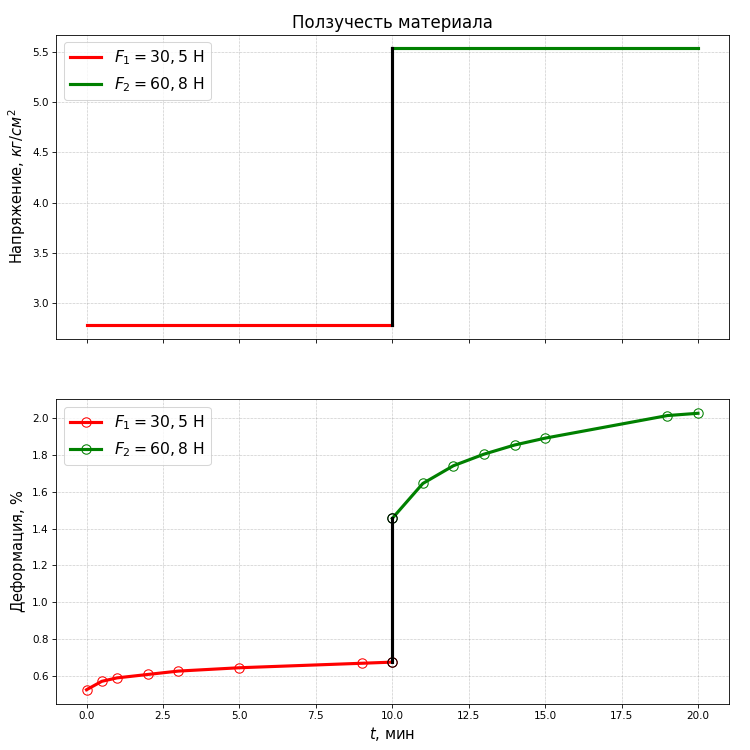
\includegraphics[width = 0.9\textwidth]{Eps and Sigm ot t.png}
\end{figure}


%\textbf{Вывод:} 

\end{document}
